\documentclass[
    pdftex,
    12pt,
    parskip=half,
    a4paper
]{scrartcl}
\author{Crawford, Sam}
\title{Einführung in Kryptographie und IT-Sicherheit}

\usepackage[utf8]{inputenc}
\usepackage[naustrian]{babel}
\usepackage{graphicx}
\usepackage{listings}
\usepackage{xcolor}
\usepackage{mathtools}
\usepackage{subcaption}

% Define color scheme
\definecolor{codeblue}{rgb}{0.13, 0.13, 0.75}
\definecolor{codegreen}{rgb}{0, 0.5, 0}
\definecolor{codered}{rgb}{0.75, 0.13, 0.13}
\definecolor{codegray}{rgb}{0.5, 0.5, 0.5}
\definecolor{backgray}{rgb}{0.95, 0.95, 0.95}

% Define Python style for listings
\lstdefinestyle{pythonstyle}{
    language=Python,
    basicstyle=\ttfamily,
    keywordstyle=\color{codeblue}\bfseries,
    stringstyle=\color{codered},
    commentstyle=\color{codegreen}\itshape,
    numberstyle=\tiny\color{codegray},
    numbers=left,
    stepnumber=1,
    numbersep=10pt,
    backgroundcolor=\color{backgray},
    showspaces=false,
    showstringspaces=false,
    frame=single,
    tabsize=3,
    breaklines=true,
    breakatwhitespace=true,
}
\lstset{style=pythonstyle}

\usepackage[naustrian]{babel}

\begin{document}
\maketitle

\section{Implementierung der Baker Map}
% \lstinputlisting[style=pythonstyle, caption=This is code]{test.py}

\section{Chaos-basierte Bildverschlüsselung und Entschlüsselung}
\subsection{Motivation}
Für die Verschlüsselung von Bildern wird eine Methode benötigt, die den Inhalt
versteckt. Bilder bestehen aus einer Struktur von Pixeln, d.h. es ist relevant welche Pixel neben welchen
Pixeln liegen. Weiters weisen Bilder eine hohe Redundanz auf. Traditionelle Verschlüsselungsmethoden beachten
diese Aspekte bei Bildern nicht wirklich und somit ist eine andere Verschlüsselungsmethode erforderlich.
Chaos-basierte Verschlüsselung ist deterministisch, hat eine hohe Ergodizidät, d.h. es werden praktisch alle
möglichen Zustände des Systems über einen längeren Zeitraum angenommen, und weist Pseudo-Zufälligkeit auf. Außerdem
sind sie sehr sensibel zu den Ausgangsbedingungen, d.h. kleine Veränderungen der Ausgangsbedingungen führen zu
sehr anderen Ergebnissen. Das bedeutet, dass aufgrund der Komplexität solcher Systeme es schwer ist,
das Verhalten vorherzusehen.
Somit sind chaos-basierte Verschlüsselungen von Vorteil für die Verschlüsselung von Bildern.
\cite{zhang2023}

\subsection{Funktionsweise}
Die chaos-basierte Verschlüsselung nutzt eine chaotische Abbildung wie die Baker Map oder Cat Map. Beide bilden
einen 2-dimensionalen Einheitsquadrat auf sich selber ab. Der Grund warum diese Abbildungen gewählt werden ist, da
sie relativ simpel sind und somit schnell verschlüsselt/enschlüsselt werden kann. 
Eine solche Abbildung wird dann im nächsten Schritt generalisiert, indem Parameter zur Abbildung hinzugefügt werden.
Danach wird sie diskretisiert, denn ein Bild besteht aus diskreten Pixeln. Das bedeutet, dass die Abbildung so
modifiziert wird, sodass sie nicht mehr ein Einheitsquadrat auf sich selbst abbilden, sondern ein 2-dimensionales quadratisches
Bild bestehend aus Pixeln auf sich selber abbildet. So eine Abbildung bestimmt also eine Bijektion zwischen den einzelnen Pixeln
quadratischer Bilder, sodass eine Permutation der Pixel berechnet werden kann. Anschließend wird die Abbildung auf 3 Dimensionen erweitert,
sodass einzelne Pixel Werte modifiziert werden. Schlussendlich wird dann eine Diffusion noch angewendet als Komposition zur bestehenden
Abbildung.
\cite{IEEEMap}

Zur Entschlüsselung wird dann die inverse Baker Map verwendet, sodass man das Ursprungsbild wieder erhaltet nach gleich vielen Iterationen.

\subsubsection{Baker Map}
Die Baker Map ist eine chaotische Abbildung des Einheitsquadrates $I \times I$ auf sich selbst, die formell folgendermaßen beschrieben wird:
$$B(x, y) = (2x, \frac{y}{2}) \text{ if } x < \frac{1}{2}$$
$$B(x, y) = (2x - 1, \frac{y + 1}{2}) \text{ if } \frac{1}{2} \leq x \leq 1$$
Wobei $x$ und $y$ die Koordinaten sind.
In Worten ist die Baker Map eine Abbildung, die einen Einheitsquadrat so auf sich selbst abbildet: Als erstes wird er vertikal in zwei Rechtecken
aufgeteilt. Dann werden diese langgestreckt, sodass die Höhe sich halbiert. Anschließend wird eine der Hälften auf die andere gelegt. Diesen
Prozess kann man mit der Arbeit eines Bäckers beim Kneten von Teig vergleichen, daher der Name.
\cite{IEEEMap}

\subsubsection{Cat Map}
Die standard Cat Map, die ein quadratisches Bild $N \times N$ auf sich selbst abbildet, ist folgendermaßen definiert:
$$
	\begin{bmatrix} x' \\ y' \end{bmatrix} =
	\begin{bmatrix} 1 & 1 \\ 1 & 2 \end{bmatrix}
	\begin{bmatrix} x \\ y \end{bmatrix} (\mod N)
$$
Wobei $x, y \in \{0, 1, \dots , N - 1 \}$, $(x, y)$ ist ein Pixel des Originalbildes und $(x', y')$ ist das abgebildete Pixel.
\cite{catmap}

\section{Verschlüsselung mit AES}
Der für die Verschlüsselung verwendete Programmcode ist folgender:
\begin{lstlisting}
import cv2
from Crypto.Cipher import AES

def encrypt_image(key, image):
    length, _ = image.shape
    flat_original = image.flatten()
    flat_encrypted = flat_original.copy()
    nonces = []

    for i in range(0, len(flat_original), 16):
        cipher = AES.new(key, AES.MODE_EAX)
        nonces.append(cipher.nonce)
        pixels = flat_original[i : i + 16]

        encrypted_bytes = cipher.encrypt_and_digest(b"".join(pixels))

        for j in range(16):
            flat_encrypted[i + j] = encrypted_bytes[j]

    encrypted_image = flat_encrypted.reshape((length, length))
    return nonces, encrypted_image

\end{lstlisting}
Die Funktion \lstinline{encrypt_image()} besitzt zwei Parameter: einen Schlüssel und natürlich das Bild,
das man verschlüsseln möchte. In \lstinline{length} wird die Seitenlänge des Bildes gespeichert. Dann wird das 2D-Bild-Array
mit \lstinline{.flatten()} zu einem 1D-Array umgewandelt, für die leichtere Handhabung. Außerdem wird ein weiteres 1D-Array
gleicher Länge angelegt, wo die verschlüsselten Pixel dann gesetzt werden.

In den Zeilen 10 bis 18 ist dann der Hauptalgorithmus. Für jede 16 Elemente des 1D-Arrays wird ein neuer Cipher erstellt,
dessen nonce in die \lstinline{nonces} Liste gespeichert wird. Anschließend werden die 16 Elemente, welche alle vom Typ uint8
sind, zu einem 128-Bit Block zusammengeführt und mithilfe dem cipher verschlüsselt. \lstinline{encrypted_bytes} sind dann
die verschlüsselten 128 Bits. Dann wird an jene Stellen, von denen die ursprünglichen Bytes kommen, die verschlüsselten
16 Bytes in das neue 1D-Array gesetzt. Nachdem der äußerste For-Loop terminiert ist, wird das neu befüllte 1D-Array in ein
Bild umgewandelt, welches dann mit den nonces als 2-Tupel zurückgegeben wird.

Zum Entschlüsseln benötigt man denselben Schlüssel und die nonces. Die Funktion dazu ist diese hier:
\begin{lstlisting}
def decrypt_image(nonces, key, image):
    length, _ = image.shape
    flat_encrypted = image.flatten()
    flat_decrypted = flat_encrypted.copy()

    for i in range(0, len(flat_encrypted), 16):
        cipher = AES.new(key, AES.MODE_EAX, nonce=nonces[i // 16])
        pixels = flat_encrypted[i : i + 16]

        decrypted_bytes = cipher.decrypt(b"".join(pixels))
        for j in range(16):
            flat_decrypted[i + j] = decrypted_bytes[j]

    return flat_decrypted.reshape((length, length))
\end{lstlisting}
Die Funktionsweise ist analog zu \lstinline{encrypt_image()}. Die 2D-Arrays werden in 1D-Arrays umgewandelt. Dann wird für alle
16 Bytes diese 16 Bytes mithilfe des Schlüssels und der nonces entschlüsselt. Anschließend werden diese entschlüsselten Bytes
bei dem neuen 1D-Array entsprechend ihrer ursprünglichen Positionen gesetzt. Als Letztes wird dann dieses entschlüsselte 1D-Array
in ein 2D-Bild-Array zurückgewandelt und man hat somit das verschlüsselte Bild entschlüsselt.

\subsection{Verschlüsseln von 10 Bildern}
Für konkrete Beispiele mit den jeweiligen Entropien, siehe Abbildungen \ref{fig:cat} bis \ref{fig:sky}.

\subsection{Zeitbedarf der Verschlüsselung}
Was den Zeitbedarf der Verschlüsselung betrifft: Die Ausführung des Programms dauert im Durchschnitt
$1.974$ Sekunden. Die Tabelle \ref{tab:speed3} gibt die konkreten Werte pro Bild an, wobei die Zahlen
die Ordnung der Bilder entsprechen.
\begin{table}
	\begin{center}
		\begin{tabular}{ |c|c|c| } 
		\hline
		Bild & Zeit (in Sekunden) \\
		\hline
		1 & 2.00 \\
		2 & 1.97\\
		3 & 1.98\\
		4 & 1.96\\
		5 & 1.96\\
		6 & 1.94\\
		7 & 1.97\\
		8 & 1.97\\
		9 & 2.01\\
		10 & 1.98\\
		\hline
		\end{tabular}
	\end{center}
	\caption{Die individuellen Zeiten um ein Bild zu verschlüsseln}
	\label{tab:speed3}
\end{table}

\begin{figure}
	\centering

	\begin{subfigure}{0.35\textwidth}
		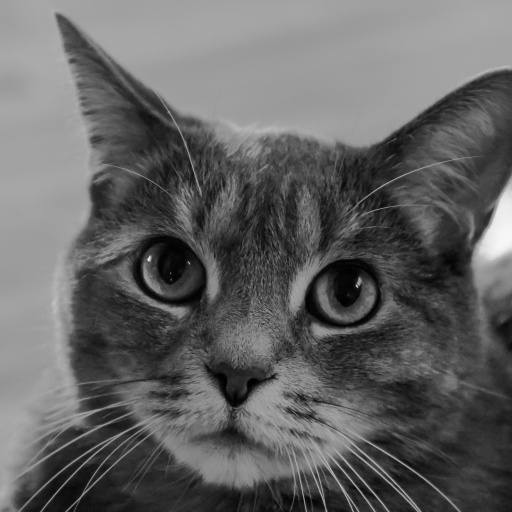
\includegraphics[width=\textwidth]{3/gray_7.055047578254635_cat.jpg}
		\caption{Entropie: 7.055047578254635}
	\end{subfigure}
	\hfill
	\begin{subfigure}{0.35\textwidth}
		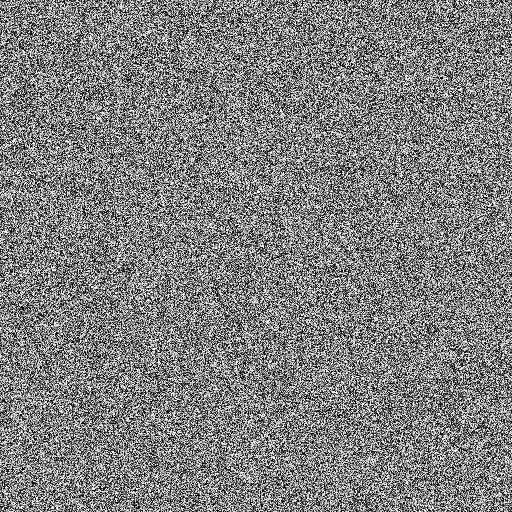
\includegraphics[width=\textwidth]{../1/3/encrypted_7.999306298374896_cat.jpg}
		\caption{Entropie: 7.999184881574807}
	\end{subfigure}

	\caption{Bild vor (links) und nach (rechts) Verschlüsselung}
	\label{fig:cat}
\end{figure}

\begin{figure}
	\centering

	\begin{subfigure}{0.35\textwidth}
		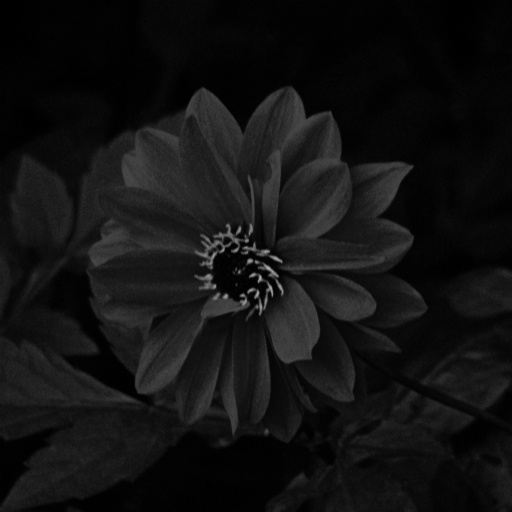
\includegraphics[width=\textwidth]{../1/3/gray_5.489817933250877_flower.jpg}
		\caption{Entropie: 5.489817933250877}
	\end{subfigure}
	\hfill
	\begin{subfigure}{0.35\textwidth}
		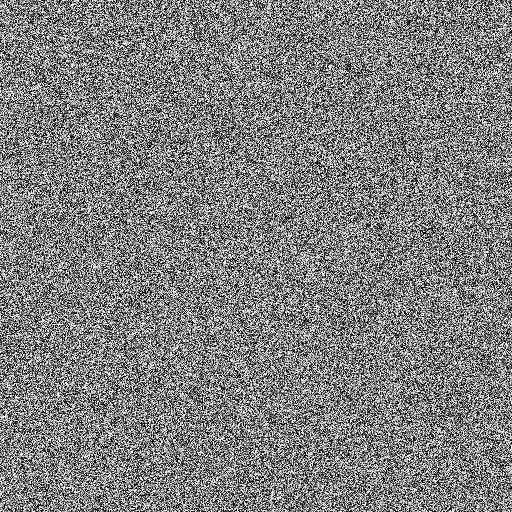
\includegraphics[width=\textwidth]{../1/3/encrypted_7.999228181754879_flower.jpg}
		\caption{Entropie: 7.999228181754879}
	\end{subfigure}

	\caption{Bild vor (links) und nach (rechts) Verschlüsselung}
	\label{fig:flower}
\end{figure}

\begin{figure}
	\centering

	\begin{subfigure}{0.35\textwidth}
		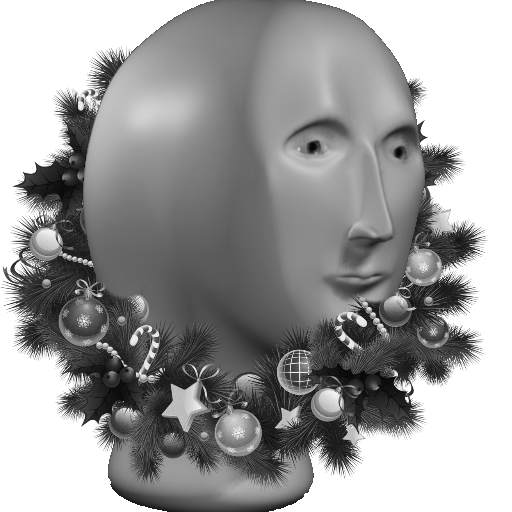
\includegraphics[width=\textwidth]{../1/3/gray_6.176106420718194_meme_man.png}
		\caption{Entropie: 6.176106420718194}
	\end{subfigure}
	\hfill
	\begin{subfigure}{0.35\textwidth}
		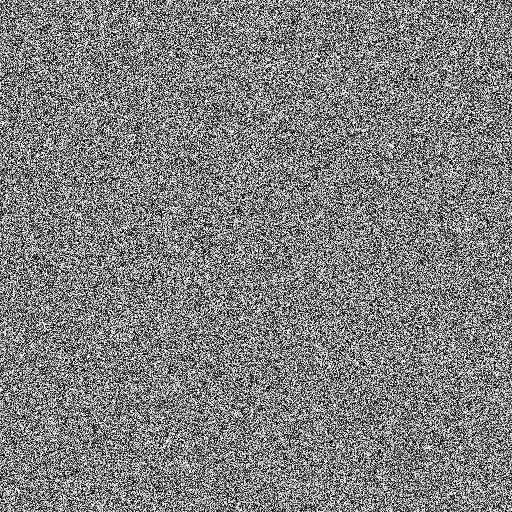
\includegraphics[width=\textwidth]{../1/3/encrypted_7.9994342031643875_meme_man.png}
		\caption{Entropie: 7.999434203164387}
	\end{subfigure}

	\caption{Bild vor (links) und nach (rechts) Verschlüsselung}
	\label{fig:meme_man}
\end{figure}

\begin{figure}
	\centering

	\begin{subfigure}{0.35\textwidth}
		
\includegraphics[width=\textwidth]{../1/3/gray_1.968975268089162_spheal.png}
		\caption{Entropie: 1.968975268089162}
	\end{subfigure}
	\hfill
	\begin{subfigure}{0.35\textwidth}
		
\includegraphics[width=\textwidth]{../1/3/encrypted_7.999230248060936_spheal.png}
		\caption{Entropie: 7.999230248060936}
	\end{subfigure}

	\caption{Bild vor (links) und nach (rechts) Verschlüsselung}
	\label{fig:spheal}
\end{figure}

\begin{figure}
	\centering

	\begin{subfigure}{0.35\textwidth}
		
\includegraphics[width=\textwidth]{../1/3/gray_4.1555418953746175_frog.jpg}
		\caption{Entropie: 4.155541895374617}
	\end{subfigure}
	\hfill
	\begin{subfigure}{0.35\textwidth}
		
\includegraphics[width=\textwidth]{../1/3/encrypted_7.99926694689182_frog.jpg}
		\caption{Entropie: 7.99926694689182}
	\end{subfigure}

	\caption{Bild vor (links) und nach (rechts) Verschlüsselung}
	\label{fig:frog}
\end{figure}

\begin{figure}
	\centering

	\begin{subfigure}{0.35\textwidth}
		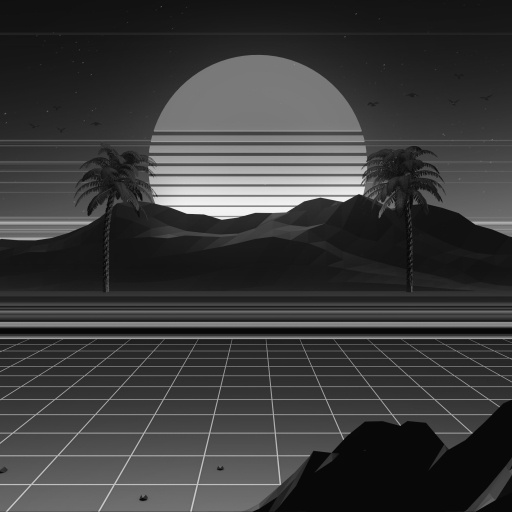
\includegraphics[width=\textwidth]{../1/3/gray_6.761302835772753_synthwave.jpg}
		\caption{Entropie: 6.761302835772753}
	\end{subfigure}
	\hfill
	\begin{subfigure}{0.35\textwidth}
		
\includegraphics[width=\textwidth]{../1/3/encrypted_7.999284747927613_synthwave.jpg}
		\caption{Entropie: 7.999284747927613}
	\end{subfigure}

	\caption{Bild vor (links) und nach (rechts) Verschlüsselung}
	\label{fig:synthwave}
\end{figure}

\begin{figure}
	\centering

	\begin{subfigure}{0.35\textwidth}
		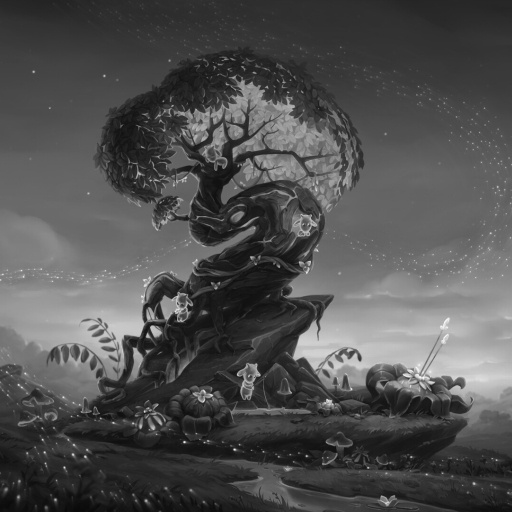
\includegraphics[width=\textwidth]{../1/3/gray_7.2193250947721515_fantasy_tree.jpg}
		\caption{Entropie: 7.219325094772151}
	\end{subfigure}
	\hfill
	\begin{subfigure}{0.35\textwidth}
		
\includegraphics[width=\textwidth]{../1/3/encrypted_7.999340174814104_fantasy_tree.jpg}
		\caption{Entropie: 7.999340174814104}
	\end{subfigure}

	\caption{Bild vor (links) und nach (rechts) Verschlüsselung}
	\label{fig:fantasy}
\end{figure}

\begin{figure}
	\centering

	\begin{subfigure}{0.35\textwidth}
		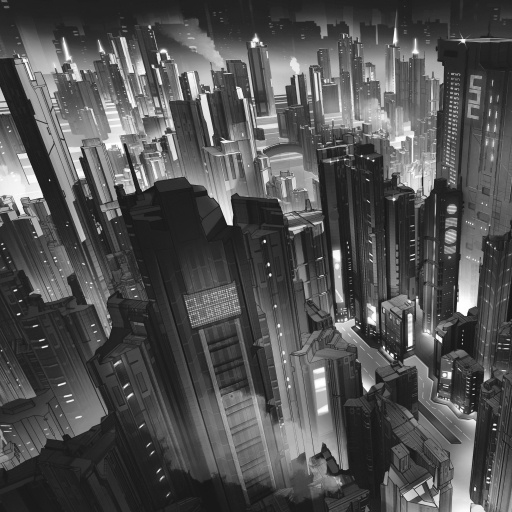
\includegraphics[width=\textwidth]{../1/3/gray_7.228465731556658_city.jpg}
		\caption{Entropie: 7.228465731556658}
	\end{subfigure}
	\hfill
	\begin{subfigure}{0.35\textwidth}
		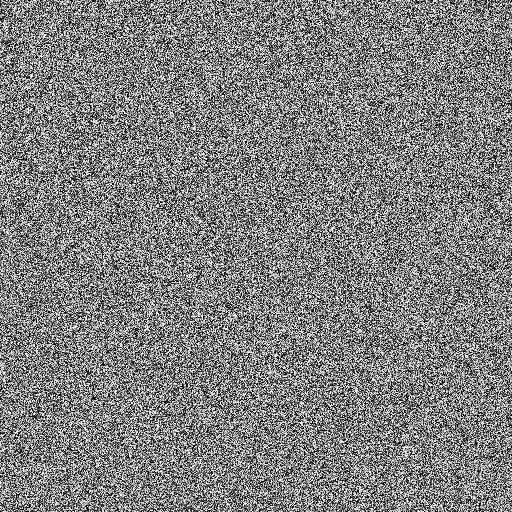
\includegraphics[width=\textwidth]{../1/3/encrypted_7.999378267461962_city.jpg}
		\caption{Entropie: 7.999378267461962}
	\end{subfigure}

	\caption{Bild vor (links) und nach (rechts) Verschlüsselung}
	\label{fig:city}
\end{figure}

\begin{figure}
	\centering

	\begin{subfigure}{0.35\textwidth}
		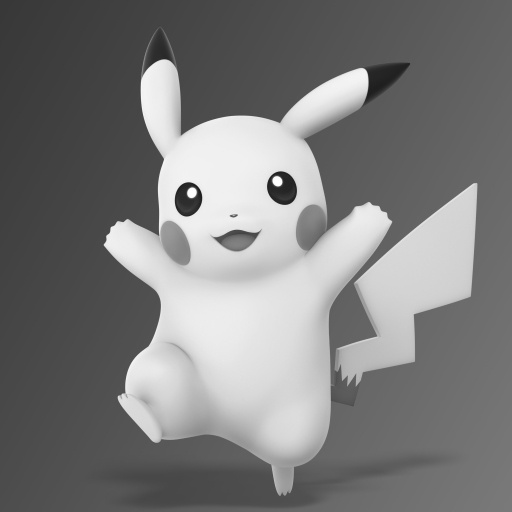
\includegraphics[width=\textwidth]{../1/3/gray_6.920844020928125_pikachu.jpg}
		\caption{Entropie: 6.920844020928125}
	\end{subfigure}
	\hfill
	\begin{subfigure}{0.35\textwidth}
		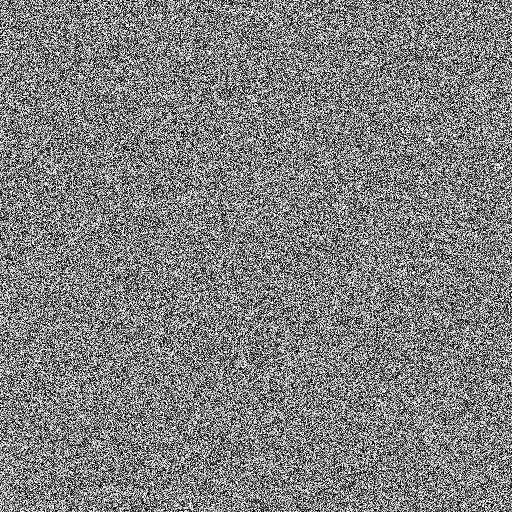
\includegraphics[width=\textwidth]{../1/3/encrypted_7.999482477476632_pikachu.jpg}
		\caption{Entropie: 7.999482477476632}
	\end{subfigure}

	\caption{Bild vor (links) und nach (rechts) Verschlüsselung}
	\label{fig:pika}
\end{figure}

\begin{figure}
	\centering

	\begin{subfigure}{0.35\textwidth}
		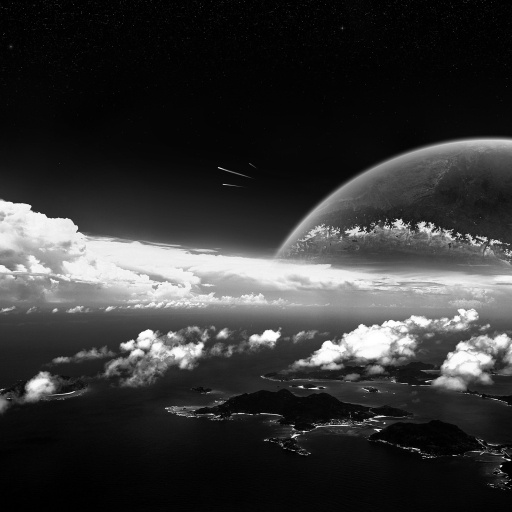
\includegraphics[width=\textwidth]{../1/3/gray_6.636128377207226_planet_sky.jpg}
		\caption{Entropie: 6.636128377207226}
	\end{subfigure}
	\hfill
	\begin{subfigure}{0.35\textwidth}
		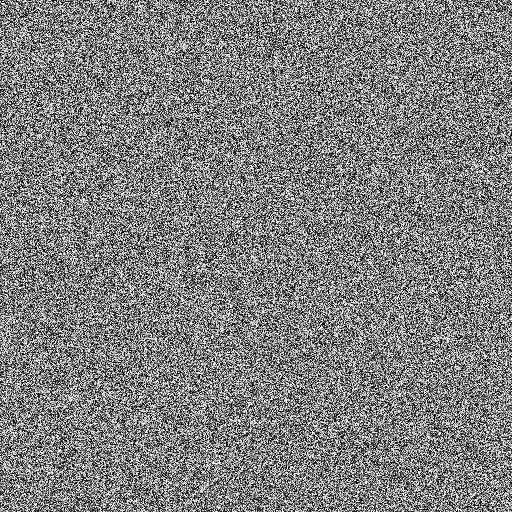
\includegraphics[width=\textwidth]{../1/3/encrypted_7.9992924900783855_planet_sky.jpg}
		\caption{Entropie: 7.999292490078385}
	\end{subfigure}

	\caption{Bild vor (links) und nach (rechts) Verschlüsselung}
	\label{fig:sky}
\end{figure}


\section{Artikel: Deprecating Motivation and Empirical Security Analysis of Chaos-based Image and Video Encryption}
Im Artikel \cite{chaos}

\section{Fehlerkorrektur mit Hammingcodes}

\bibliography{lit}
\bibliographystyle{alpha}
\end{document}
